
% \titlegraphic{\hfill\includegraphics[height=1.5cm]{logo.pdf}}

\documentclass[xcolor=pdftex,dvipsnames,table,numbers,hyperref={pdfpagelabels=false},compress]{beamer}
%\usepackage{requiredPackage}
\usepackage{amsmath}
\usepackage{graphicx}
\usepackage{amsfonts}
\usepackage{amssymb}

\usepackage{tabularx}
\usepackage{epstopdf}
\usepackage{overpic}
\usepackage{url}
\usepackage{calrsfs}
\usepackage{mathrsfs}
\usepackage{epsfig}
\usepackage{cancel}
\usepackage{changepage}

\usepackage{tikz}
\usepackage[customcolors]{hf-tikz} 

\usepackage{lmodern}
%\usepackage{mystyle}
\usepackage{subfig}
\usepackage{pifont}
\usepackage{tabu}
\usepackage{xcolor}
\usepackage{algorithm}
\usepackage{algpseudocode}
%\usepackage{enumitem}
\usepackage{remreset}
\usepackage{etoolbox}
\usepackage{comment} % end and begin comment
%\usepackage{dtklogos} 
\usepackage{listings}
\lstset{breaklines=true} 

\newcommand{\gline}{\textcolor{gray}{\hline}}
\newcommand{\cmark}{\ding{51}}%
\newcommand{\xmark}{\ding{55}}%
\newcommand{\gcheck}{\textcolor{blue}{\Large \cmark}}
\newcommand{\rcross}{\textcolor{red}{\Large \xmark}}
\newcommand{\tkt}{\tilde{K}_\theta}
\newcommand{\kt}{K_\theta}
\newcommand{\ind}{\overset{ind}{\sim}}
\newcommand{\plim}{\overset{p}{\rightarrow}}
\newcommand{\cx}{\frac {X'X}n}
\newcommand{\cz}{\frac {Z'Z}n}
\newcommand{\ccz}{\frac {Z'Z}n - \Sigma_A}
\newcommand{\czy}{\frac {Z'y}n}
\newcommand{\cyz}{\frac {y'Z}n}
\newcommand{\cxy}{\frac {X'y}n}
\newcommand{\cyx}{\frac {y'X}n}
\newcommand{\myitem}{\vskip3mm \item}

\newcommand{\calS}{{\cal S}}
\newcommand{\calA}{{\cal A}}
\newcommand{\calK}{{\cal K}}
\newcommand{\calX}{{\cal X}}
\newcommand{\calD}{{\cal D}}
\newcommand{\calG}{{\cal G}}
\newcommand{\calT}{{\cal T}}
\newcommand{\calU}{{\cal U}}
\newcommand{\calR}{{\cal R}}
\newcommand{\tp}{\tilde{p}}
\newcommand{\tildebC}{\tilde{\bC}}
\newcommand{\calL}{{\cal L}}

\newcommand{\blam}{ \mbox{\boldmath $ \lambda $} }
\newcommand{\bet}{ \mbox{\boldmath $ \eta $} }
\newcommand{\bome}{ \mbox{\boldmath $ \omega $} }
\newcommand{\bbet}{ \mbox{\boldmath $ \beta $} }
\newcommand{\bbeta}{ \mbox{\boldmath $ \beta $} }
\newcommand{\balph}{ \mbox{\boldmath $ \alpha $} }
\newcommand{\balpha}{ \mbox{\boldmath $ \alpha $} }
\newcommand{\bphi}{ \mbox{\boldmath $\phi$}}
\newcommand{\bzeta}{ \mbox{\boldmath $\zeta$}}
\newcommand{\bkap}{ \mbox{\boldmath $\kappa$}}
\newcommand{\bkappa}{ \mbox{\boldmath $\kappa$}}
\newcommand{\beps}{ \mbox{\boldmath $\epsilon$}}
\newcommand{\bepsilon}{ \mbox{\boldmath $\epsilon$}}
\newcommand{\bthet}{ \mbox{\boldmath $ \theta $} }
\newcommand{\btheta}{ \mbox{\boldmath $ \theta $} }
\newcommand{\blambda}{ \mbox{\boldmath $ \lambda $} }
\newcommand{\bnu}{ \mbox{\boldmath $\nu$} }
\newcommand{\bmu}{ \mbox{\boldmath $\mu$} }
\newcommand{\bGam}{ \mbox{\boldmath $\Gamma$} }
\newcommand{\bSig}{ \mbox{\boldmath $\Sigma$} }
\newcommand{\bSigma}{ \mbox{\boldmath $\Sigma$} }
\newcommand{\bPhi}{ \mbox{\boldmath $\Phi$} }
\newcommand{\bThet}{ \mbox{\boldmath $\Theta$} }
\newcommand{\bTheta}{ \mbox{\boldmath $\Theta$} }
\newcommand{\bDel}{ \mbox{\boldmath $\Delta$} }
\newcommand{\bDelta}{ \mbox{\boldmath $\Delta$} }
\newcommand{\bnabla}{ \mbox{\boldmath $\nabla$} }
\newcommand{\bLam}{ \mbox{\boldmath $\Lambda$} }
\newcommand{\bLambda}{ \mbox{\boldmath $\Lambda$} }
\newcommand{\bgam}{ \mbox{\boldmath $\gamma$} }
\newcommand{\bgamma}{ \mbox{\boldmath $\gamma$} }
\newcommand{\brho}{ \mbox{\boldmath $\rho$} }
\newcommand{\bdel}{ \mbox{\boldmath $\delta$} }
\newcommand{\bdelta}{ \mbox{\boldmath $\delta$} }
\newcommand{\sis}{\sigma^2}
\newcommand{\bOmega}{\mbox{\boldmath $\Omega$} }
\newcommand{\bPsi}{ {\boldsymbol \Psi} }
\newcommand{\btkt}{\boldsymbol{\tilde{K}}_\theta}
\newcommand{\pg}{P{\'o}lya-Gamma }

\newcommand{\bzero}{\textbf{0}}
\newcommand{\bones}{\textbf{1}}
\newcommand{\ba}{\textbf{a}}
\newcommand{\bb}{\textbf{b}}
\newcommand{\bB}{\textbf{B}}
%\newcommand{\bA}{\textbf{A}}
\newcommand{\bc}{\textbf{c}}
\newcommand{\bC}{\textbf{C}}
\newcommand{\bA}{\textbf{A}}
\newcommand{\bd}{\textbf{d}}
\newcommand{\bD}{\textbf{D}}
\newcommand{\be}{\textbf{e}}
\newcommand{\bE}{\textbf{E}}
\newcommand{\bk}{\textbf{k}}
\newcommand{\bK}{\textbf{K}}
\newcommand{\bh}{\textbf{h}}
\newcommand{\bs}{\textbf{s}}
\newcommand{\bS}{\textbf{S}}
\newcommand{\bH}{\textbf{H}}
\newcommand{\bI}{\textbf{I}}
\newcommand{\bt}{\textbf{t}}
\newcommand{\bu}{\textbf{u}}
\newcommand{\bv}{\textbf{v}}
\newcommand{\bw}{\textbf{w}}
\newcommand{\bW}{\textbf{W}}
\newcommand{\bx}{\textbf{x}}
\newcommand{\bX}{\textbf{X}}
\newcommand{\by}{\textbf{y}}
\newcommand{\bY}{\textbf{Y}}
\newcommand{\bz}{\textbf{z}}
\newcommand{\bZ}{\textbf{Z}}
\newcommand{\bL}{\textbf{L}}
\newcommand{\br}{\textbf{r}}
\newcommand{\bR}{\textbf{R}}
\newcommand{\bm}{\textbf{m}}
\newcommand{\bM}{\textbf{M}}
\newcommand{\given}{\,|\,}
\newcommand{\T}{\top}
\newcommand{\bV}{\textbf{V}}
\newcommand{\bJ}{\textbf{J}}
\newcommand{\blue}[1]{{\color{RoyalBlue!90} #1}}
\newcommand{\red}[1]{{\color{Red} #1}}
\newcommand{\green}[1]{{\color{Green} #1}}
\newcommand{\orange}[1]{{\color{Orange} #1}}
\newcommand{\titl}[1]{{\begin{large}\begin{center}#1\end{center}\end{large}}}

\newcommand{\tildea}{\tilde{a}}
\newcommand{\tildeba}{\tilde{\ba}}
\newcommand{\tildebv}{\tilde{\bv}}
\newcommand{\tildev}{\tilde{v}}
\newcommand{\tildeA}{\tilde{A}}
\newcommand{\tildeC}{\tilde{C}}
\newcommand{\tildeK}{\tilde{K}}
\newcommand{\tildew}{\tilde{w}}
\newcommand{\tildeu}{\tilde{u}}
\newcommand{\tildebw}{\tilde{\bw}}
\newcommand{\tildeeps}{\tilde{\epsilon}}
\newcommand{\tildebeps}{\tilde{\bepsilon}}
\newcommand{\eps}{\epsilon}
\newcommand{\sigs}{\sigma^2}
\newcommand{\taus}{\tau^2}
\newcommand{\iid}{\stackrel{\mathrm{iid}}{\sim}}

%\newcommand{\calS}{{\cal S}}
\newcommand{\calC}{{\cal C}}

%\documentclass[10pt]{beamer}

\usetheme{metropolis}
\usepackage{appendixnumberbeamer}

\usepackage{booktabs}
\usepackage[scale=2]{ccicons}

\usepackage{pgfplots}
\usepgfplotslibrary{dateplot}

\usepackage{xspace}
\newcommand{\themename}{\textbf{\textsc{metropolis}}\xspace}

\makeatletter
\@addtoreset{subfigure}{framenumber}% subfigure counter resets every frame
\makeatother

\makeatletter
\@addtoreset{figure}{framenumber}% subfigure counter resets every frame
\makeatother

\setbeamertemplate{caption}{\raggedright\insertcaption\par}
\captionsetup[subfigure]{labelformat=empty}




\title[]{Low-Rank and Predictive Process Models}
\author{Andrew Finley$^1$ \& Jeffrey Doser$^2$}
	
\institute{
\begin{tiny}$^1$Department of Forestry, Michigan State University.\\
$^2$Department of Integrative Biology, Michigan State University.\end{tiny}
}

\date{May 15, 2023}


\begin{document}

\maketitle


\begin{frame}{Multivariate Gaussian likelihoods for geostatistical models}

 \begin{itemize}\setlength{\itemsep}{0.4cm}
  \item $\calL=\{s_1,s_2,\ldots,s_n\}$ are locations where data is observed
  \item $y(s_i)$ is outcome at the $i$-th location, $y=(y(s_1),y(s_2),\ldots,y(s_n))^{\top}$ 
  \item Model: $y \sim N(X\beta, K_{\theta})$
  \item Estimating process parameters from the likelihood:
  \[
   -\frac{1}{2}\log\det(K_{\theta}) - \frac{1}{2}(y-X\beta)^{\top}K_{\theta}^{-1}(y-X\beta)
  \]
%  \item Customary: $K_\theta = C_{(\sigma,\phi)} + D_{\tau}$, where $\theta = \{\sigma,\phi,\tau\}$
    \item $K_{\theta}$ is usually dense with no exploitable structure
  \item Bayesian inference: Priors on $\{\beta,\theta\}$
  \item Challenges: Storage and $\texttt{chol}(K_{\theta}) = LDL^{\top}$.
 \end{itemize}

\end{frame}

\begin{frame}{Prediction and interpolation}

 \begin{itemize}\setlength{\itemsep}{0.75cm}
  \item Conditional predictive density 
\begin{align*}
% p(y(s_0)\given y, \theta, \beta) =& N\left\{y(s_0) \left| \begin{array}{l}
%                                      x^{\T}(s_0)\beta + k_{\theta}^{\T}(s_0)K^{-1}_{\theta}(y-X\beta)\;, \\
%                                      \qquad K_{\theta}(s_0,s_0) - k_{\theta}^{\T}(s_0)K^{-1}_{\theta}k_{\theta}(s_0)
%                                    \end{array}
%                                    \right.\right\}
%% & N\left\{\left. y(s_0) \right| x^{\T}(s_0)\beta + k_{\theta}^{\T}(s_0)K^{-1}_{\theta}(y-X\beta), \right. \\ 
%% & \qquad \qquad \qquad \left. K_{\theta}(s_0,s_0) - k_{\theta}^{\T}(s_0)K^{-1}_{\theta}k_{\theta}(s_0)\right\}
p(y(s_0)\given y, \theta, \beta) &= N\left(y(s_0)\left| \mu(s_0), \sigma^2(s_0)\right.\right)\;.
%\mu(s_0) &= x^{\T}(s_0)\beta + k_{\theta}^{\T}(s_0)K^{-1}_{\theta}(y-X\beta)\;, \\
%\sigma^2(s_0) &= K_{\theta}(s_0,s_0) - k_{\theta}^{\T}(s_0)K^{-1}_{\theta}k_{\theta}(s_0)\; . 
\end{align*}

\item ``Kriging'' (spatial prediction/interpolation)
\begin{align*}
 \mu(s_0) &= \mbox{E}[y(s_0)\given y,\theta] = x^{\top}(s_0)\beta + k_{\theta}^{\top}(s_0)K^{-1}_{\theta}(y-X\beta)\;, \\
 \sigma^2(s_0) &= \mbox{var}[y(s_0)\given y,\theta] = K_{\theta}(s_0,s_0) - k_{\theta}^{\top}(s_0)K^{-1}_{\theta}k_{\theta}(s_0)\; .  
\end{align*}
 
  \item Bayesian ``kriging'' computes (simulates) posterior predictive density:
\[
 p(y(s_0)\given y) = \int p(y(s_0)\given y, \theta, \beta) p(\beta, \theta \given y) \mbox{d}\beta\mbox{d}\theta  
\]
  
 \end{itemize}

\end{frame}

\begin{frame}{Computational Details}
 
 \begin{itemize}\setlength{\itemsep}{0.4cm}
  \item Compute the mean and variance (for any given $\{\beta, \theta\}$ and $s_0$):
  \begin{align*}
  \begin{array}{lc}
  \mbox{Solve for $u$: } & K_{\theta}u = k_{\theta}(s_0)\;; \\
  \mbox{Predictive mean: } & x^{\T}(s_0)\beta + u^{\top}(y - X\beta)\;; \\
  \mbox{Predictive variance: } & K_{\theta}(s_0,s_0) - u^{\top}k_{\theta}(s_0)\;.
  \end{array}
  \end{align*}
  
  \item Compute the mean and variance (for any given $\{\beta, \theta\}$ and $s_0$):
  \begin{align*}
  \begin{array}{lc}
  \mbox{Cholesky: } & \texttt{chol}(K_{\theta}) = LDL^{\top}\;; \\
  \mbox{Solve for $v$: } & v = \texttt{trsolve}(L, k_{\theta}(s_0))\;;\\ 
  \mbox{Solve for $u$: } & u = \texttt{trsolve}(L^{\top}, D^{-1}v)\;;\\ 
  \mbox{Predictive mean: } & x^{\T}(s_0)\beta + u^{\top}(y - X\beta)\;; \\
  \mbox{Predictive variance: } & K_{\theta}(s_0,s_0) - u^{\top}k_{\theta}(s_0)\;.
  \end{array}
  \end{align*}
  
  \item Primary bottleneck is \text{chol}$(\cdot)$
 \end{itemize}
 
\end{frame}

\begin{frame}{Burgeoning literature on spatial big data}

{\small
\begin{itemize}\setlength{\itemsep}{0.cm}
\item Low-rank models (Wahba,\ 1990; Higdon,\ 2002; Kamman \& Wand,\ 2003; Paciorek,\ 2007; Rasmussen \& Williams, 2006; Stein\ 2007,\ 2008; Cressie \& Johannesson, 2008; Banerjee et al.,\ 2008; 2010; Gramacy \& Lee 2008; Sang et al., 2011, 2012; Lemos et al., 2011; Guhaniyogi et al., 2011, 2013; Salazar et al., 2013; Katzfuss, 2016) 

\item Spectral approximations and composite likelihoods: (Fuentes 2007; Paciorek, 2007; Eidsvik et al. 2016)

%\item Composite likelihoods (Eidsvik et al. 2016)

\item Multi-resolution approaches (Nychka, 2002; Johannesson et al., 2007; Matsuo et al., 2010; Tzeng \& Huang, 2015; Katzfuss, 2016)

\item Sparsity: (Solve $Ax=b$ by (i) sparse $A$, or (ii) sparse $A^{-1}$)
\begin{enumerate}
 \item Covariance tapering (Furrer et al.\ 2006; Du et al.\ 2009; Kaufman et al.,\ 2009; Shaby and Ruppert, 2013)

 \item GMRFs to GPs: \texttt{INLA} (Rue et al. 2009; Lindgren et al., 2011)

 \item LAGP (Gramacy et al. 2014; Gramacy and Apley, 2015)

 \item Nearest-neighbor models (Vecchia 1988; Stein et al. 2004; Stroud et al 2014; Datta et al., 2016)
\end{enumerate}

\end{itemize}
}
\end{frame}

\begin{frame}{Bayesian low rank models}

\begin{itemize}\setlength{\itemsep}{0.4cm}
\item A \emph{low rank} or \emph{reduced rank} process approximates a \emph{parent} process over a smaller set of points (\emph{knots}).

\item Start with a \emph{parent process} $w(s)$ and construct $\tildew(s)$
\begin{equation*}\label{eq:generic_low_rank}
w(s) \approx \tilde{w}(s) = \sum_{j=1}^{r} b_{\theta}(s,s_{j}^{*}) z(s_{j}^{*}) = b_{\theta}^{\T}(s)z,
\end{equation*}
where 
\begin{itemize}\setlength{\itemsep}{0.25cm}
 \item $z(s)$ is \emph{any} well-defined process (could be same as $w(s)$);
 \item $b_{\theta}(s,s')$ is a family of basis functions indexed by parameters $\theta$;
 \item $\{s_1^*,s^*_2,\ldots,s^*_r\}$ are the knots;
 \item $b_{\theta}(s)$ and $z$ are $r\times 1$ vectors with components $b_{\theta}(s,s_{j}^{*})$ and $z(s_j^*)$, respectively.
\end{itemize}

\end{itemize}

\end{frame}


\begin{frame}{Bayesian low rank models (contd.)}

\begin{itemize}\setlength{\itemsep}{0.cm}
\item $\tilde{w} = (\tilde{w}(s_1), \tilde{w}(s_2),\ldots,\tilde{w}(s_{n}))^{\T}$ is represented as $\tildew = B_{\theta}z$
\item $B_{\theta}$ is $n\times r$ with $(i,j)$-th element $b_{\theta}(s_i,s_{j}^{*})$
\item Irrespective of how big $n$ is, we now have to work with the $r$ (instead of $n$) $z(s_j^*)$'s and the  $n\times r$ matrix $B_{\theta}$. 
\item Since $r << n$, the consequential dimension reduction is evident.
\item $\tildew$ is a valid stochastic process in $r$-dimensions space with covariance:
\[
 \mbox{cov}(\tilde{w}(s), \tilde{w}(s')) = b_{\theta}^{\T}(s)V_{z}b_{\theta}(s')\;,
\]
where $V_z$ is the variance-covariance matrix (also depends upon parameter $\theta$) for $z$.
\item When $n > r$, the joint distribution of ${\tilde{w}}$ is singular.
\end{itemize}

\end{frame}

\begin{frame}{The Sherman-Woodbury-Morrison formulas}

\begin{itemize}\setlength{\itemsep}{0.cm}
\item Low-rank dimension reduction is similar to Bayesian linear regression

\item Consider a simple hierarchical model (with $\beta = 0$):
\[
 N(z\given 0, V_z) \times N(y\given B_{\theta}z, D_{\tau})\; ,
\]
where $y$ is $n\times 1$, $z$ is $r\times 1$, $D_{\tau}$ and $V_z$ are positive definite matrices of sizes $n\times n$ and $r\times r$, respectively, and $B_{\theta}$ is $n\times r$.

\item The low rank specification is $B_{\theta}z$ and the prior on $z$.

\item $D_{\tau}$ (usually diagonal) has the residual variance components.

\item Computing $\mbox{var}(y)$ in two different ways yields
\[
 (D_{\tau} + B_{\theta}V_zB_{\theta}^{\T})^{-1} = D_{\tau}^{-1} - D_{\tau}^{-1}B_{\theta}(V_z^{-1} + B_{\theta}^{\T}D_{\tau}^{-1}B_{\theta})^{-1}B_{\theta}^{\T}D_{\tau}^{-1}\; .
\]

\item A companion formula for the determinant:
\[
 \det(D_{\tau} + B_{\theta}V_zB_{\theta}^{\T}) =  \det(V_z)\det(D_{\tau})\det(V_z^{-1} + B_{\theta}^{\T}D_{\tau}^{-1}B_{\theta})\;. 
\]

\end{itemize}

\end{frame}

\begin{frame}{Practical implementation for Bayesian low rank models}

\begin{itemize}\setlength{\itemsep}{0.cm}
\item In practical implementation, better to avoid SWM formulas.
 \begin{align*}\label{eq: Normal_Normal_Linear_Model}
 \begin{array}{ccccc}
  \underbrace{\begin{bmatrix} D_{\tau}^{-1/2}y \\ 0\end{bmatrix}} & = & \underbrace{\begin{bmatrix} D_{\tau}^{-1/2} B_{\theta} \\ V_z^{-1/2} \end{bmatrix}}{z} & + & \underbrace{\begin{bmatrix} e_1 \\ e_2\end{bmatrix}} \\
  y_{\ast} &  & B_{\ast} & & e_{\ast} 
 \end{array}\;.
 \end{align*}
\item $e_{\ast} \sim N(0, I_{n+r})$. 
 
\item $V_z^{1/2}$ and $D_{\tau}^{1/2}$ are matrix square roots of of $V_z$ and $D_{\tau}$, respectively. 

\item If $D_{\tau}$ is diagonal (as is common), then $D_{\tau}^{1/2}$ is simply the square root of the diagonal elements of $D_{\tau}$. 

\item $V_z^{1/2} = \texttt{chol}(V_z)$ is the triangular (upper or lower) Cholesky factor of the $r\times r$ matrix $V_{z}$. 

\item Use \texttt{backsolve} to efficiently obtain $V_z^{-1/2}z$ 

% \item The marginal density of $p(y_{\ast}\given \theta,\tau)$ after integrating out $z$ now corresponds to 
% \[
% y_{\ast} = B_{\ast}\hat{z} + e_{\ast}\;, 
% \]
% where $\hat{z}$ is the ordinary least-square estimate of $z$. 
% 
% \item Use \texttt{lm} function to compute $\hat{z}$ applying the QR decomposition to $B_{\ast}$.
\end{itemize}

\end{frame}

\begin{frame}{Practical implementation for Bayesian low rank models (contd.)}

\begin{itemize}\setlength{\itemsep}{0.cm}
\item The marginal density of $p(y_{\ast}\given \theta,\tau)$ after integrating out $z$ now corresponds to the normal linear model
\[
y_{\ast} = B_{\ast}\hat{z} + e_{\ast}\;, 
\]
where $\hat{z}$ is the ordinary least-square estimate of $z$. 

\item Use \texttt{lm} function to compute $\hat{z}$ applying the QR decomposition to $B_{\ast}$.

\item Thus, we estimate the Bayesian linear model
\[
 p(\theta,\tau) \times N(y_{\ast}\given B_{\ast}\hat{z}, I_{n+r})
\]

\item MCMC will generate posterior samples for $\{\theta, \tau\}$. 

\item \emph{Recover} the posterior samples for $z$ from those of $\{\theta,\tau\}$:
\[
 p(z\given y) = \int N(z\given \hat{z}, M) \times p(\theta,\tau\given y)\mbox{d}{\theta}\mbox{d}\tau
\]
where $M^{-1} = V_z^{-1} + B_{\theta}^{\top}D_{\tau}^{-1}B_{\theta}$.
% \[
%  p(z\given y) = \int N(z\given Mm, M) \times p(\theta,\tau\given y)\mbox{d}{\theta}\mbox{d}\tau
% \]
% where $M^{-1} = V_z^{-1} + B_{\theta}^{\top}D_{\tau}^{-1}B_{\theta}$ and $m = B_{\theta}^{\top}D_{\tau}^{-1}y$.
% \begin{align*}
%  M^{-1} &= V_z^{-1} + B_{\theta}^{\top}D_{\tau}^{-1}B_{\theta}\\
%  m &= B_{\theta}^{\top}D_{\tau}^{-1}y
% \end{align*}

\end{itemize}

\end{frame}


\begin{frame}{Predictive process models (Banerjee et al., \emph{JRSS-B}, 2008)}

\begin{itemize}\setlength{\itemsep}{0.4cm}
\item A particular low-rank model emerges by taking 
\begin{itemize}\setlength{\itemsep}{0.25cm}
 \item $z(s) = w(s)$
 \item $z = (w(s_1^*), w(s_2^*),\ldots, w(s_r^*))^{\top}$ as the realizations of the parent process $w(s)$ over the set of knots $\calL^* = \{s_1^*, s_2^*, \ldots, s_r^*\}$,
\end{itemize}
and then taking the conditional expectation:
\[
 \tildew(s)= \mbox{E}[w(s)\given w^{\ast}] = b_{\theta}^{\top}(s)z\; .
\]

\item The basis functions are \emph{automatically} derived from the spatial covariance structure of the parent process $w(s)$:
\[
b_{\theta}^{\top}(s) = \mbox{cov}\{w(s), w^{\ast}\}\mbox{var}^{-1}\{w^{\ast}\} = K_{\theta}(s,\calL^*)K_{\theta}^{-1}(\calL^*, \calL^*) \;.
\]

\end{itemize}

\end{frame}


\begin{frame}{Biases in low-rank models}

\begin{itemize}\setlength{\itemsep}{0.cm}
\item In low-rank processes, $w(s) = \tildew(s) + \eta(s)$. What is lost in $\eta(s)$?

\begin{center}
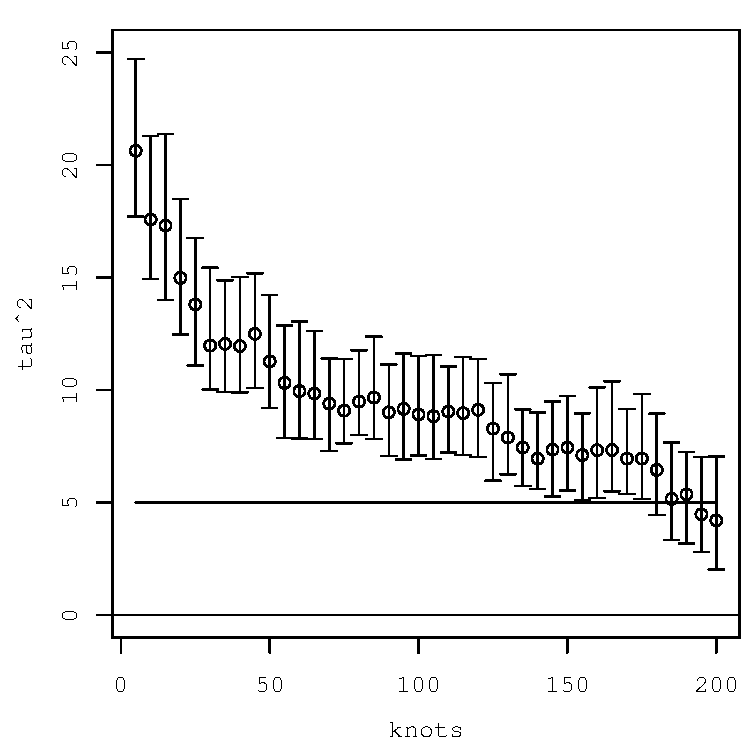
\includegraphics[width=.5\textwidth, height=.5\textheight]{../figures/n200_knots_by_5_tauSq.pdf}
\end{center}

\item For the predictive process,
\begin{align*}\label{eq: predictive_process_bias_inequality}
 \mbox{var}\{w(s)\} &= \mbox{var}\{\mbox{E}[w(s)\given w^*]\} + \mbox{E}\{\mbox{var}[w(s)\given w^*]\} \\
& \geq \mbox{var}\{\mbox{E}[w(s)\given w^*]\}\; .
\end{align*}

\end{itemize}

\end{frame}

\begin{frame}{Bias-adjusted or modified predictive processes}
 
 \begin{itemize}
  \item $\eta(s)$ is a Gaussian process with covariance structure 
\begin{align*}
 \mbox{Cov}\{\eta(s), \eta(s')\} &= K_{\eta, \theta}(s,s') \\
  &= K_{\theta}(s,s') - K_{\theta}(s, \calL^*)K_{\theta}^{-1}(\calL^*,\calL^*)K_{\theta}(\calL^*,s')\; .
\end{align*}

  \item Remedy:
\begin{equation*}\label{wq: modified_predictive_process}
 \tildew_{\epsilon}(s) = \tildew(s) + \tilde{\epsilon}(s)\; ,
\end{equation*}
where $\tilde{\epsilon}(s)\stackrel{ind}{\sim} N(0,\delta^2(s))$ and 
\[
 \delta^2(s) = \mbox{var}\{\eta(s)\} = K_{\theta}(s,s) - K_{\theta}(s, \calL^*)K_{\theta}^{-1}(\calL^*,\calL^*)K_{\theta}(\calL^*,s)\; .
\]

 \item Other improvements suggested by Sang et al. (2011, 2012) and Katzfuss (2017).

\end{itemize}
 
\end{frame}

\begin{frame}{Oversmoothing in low rank models}
 
\begin{figure}[t]
\begin{center}
\subfloat[True w]{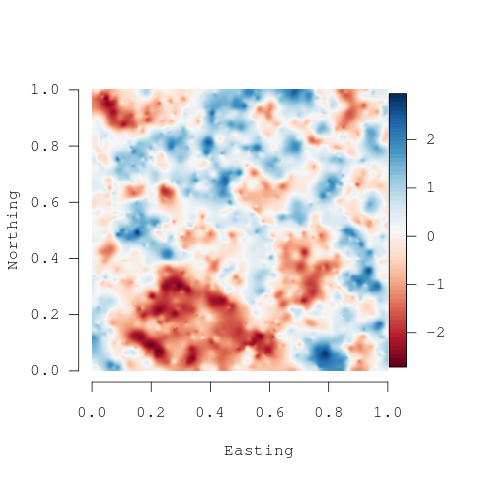
\includegraphics[width=3.5cm]{../figures/w-obs.png}\label{uni-w-obs}}
\subfloat[Full GP]{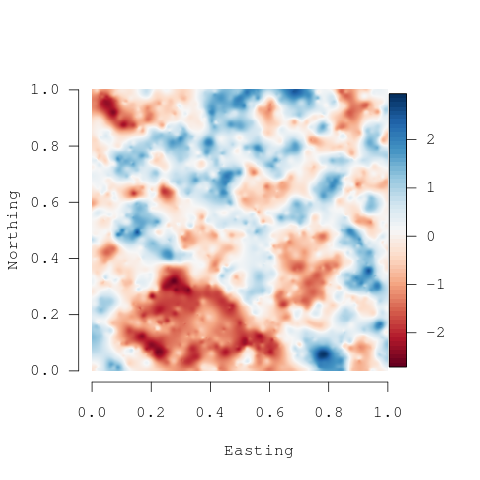
\includegraphics[width=3.5cm]{../figures/w-gs.png}\label{uni-w-gs}}
\subfloat[PPGP 64 knots]{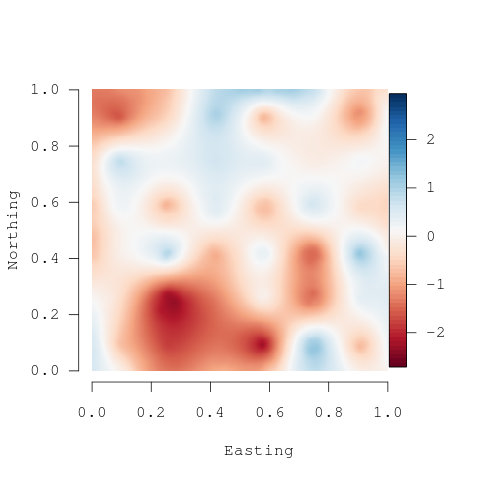
\includegraphics[width=3.5cm]{../figures/w-pp64.png}\label{uni-pp64-gs}}\\
\end{center}
\caption{Comparing full GP vs low-rank GP with 2500 locations. Figure (\ref{uni-pp64-gs}) exhibits oversmoothing by a low-rank process (predictive process with 64 knots)} %\label{fig:uni-w}
\end{figure}
 
\end{frame}


\end{document}
